\documentclass{article}

% Language setting
% Replace `english' with e.g. `spanish' to change the document language
\usepackage[portuguese]{babel}

% Set page size and margins
% Replace `letterpaper' with`a4paper' for UK/EU standard size
\usepackage[letterpaper,top=2cm,bottom=2cm,left=3cm,right=3cm,marginparwidth=1.75cm]{geometry}

% Useful packages
\usepackage{amsmath}
\usepackage{graphicx}
\usepackage[colorlinks=true, allcolors=blue]{hyperref}

\title{Avaliação Individual 2}
\author{Ramiro Berneira Nascimento\thanks{ramirobnascimento@hotmail.com}}

\begin{document}
\maketitle

\begin{abstract}
This scientific paper was proposed as the Final Individual Assessment Activity from the Languages, Automates and Computation class ministered by professor Diego Vrague Noble, at the first semester of Software Engineering in PUCRS University. The main goal of this activity is develop the knowledge of the following topics, Turing Universal Machine and Regular Grammar.  
\end{abstract}

\section{Introdução}

    Neste artigo, serão aprofundados e dissertados dois tópicos distintos. Máquina de Turing Universal e a resolução de um problema envolvendo Gramática Regular.  
    
    Para que se possa entender e definir uma Maquina de Turing Universal, será necessário abordar outros sub-tópicos primeiro, como a definição de uma maquina de Turing, qual a importância da definição desta maquina para a computação, com quais elementos uma máquina de turing é definida e como ela opera. Com este conjunto de elementos, esta máquina lê os símbolos de uma posição da fita, decide o que vai escrever nesta posição e para qual lado a fita será movida para repetir o processo. Durante esse processo, o estado Q da máquina vai mudando até chegar ou não a um estado final, tornando a palavra de entrada (valores da fita), um programa aprovado ou rejeitado.
    
    O segundo problema proposto nesta avaliação é a solução do seguinte problema:
    Uma Gramática Regular (GR) é uma gramática onde todas as regras são da forma A → aB ou A → b onde A e B são variáveis quaisquer e a e b são terminais quaisquer. O conjunto de linguagens geradas por GRs é o conjunto de linguagens regulares. Portanto, qualquer GR pode ser convertida em um Autômato FInito Não-Determinístico (AFND) que aceita a  mesma linguagem gerada pela GR. Dada GR abaixo, converta-a para um AFND que aceite a mesma linguagem e explique os passos feitos na forma de um algoritmo:
    
    $G = ({A,B}, {a,b,c,d}, R, A)$ a relação R é definida pelas seguintes produções:
    
                             \[A \longrightarrow aB | aA\] 
                            \[B \longrightarrow bB | aA | cA | d\]
                     
    
    
    
    

\section{Máquina de Turing Universal}

    Alan Turing foi um matemático britânico que estava em busca da prova matemática de que o problema proposto por David Hilbert e Wilhelm Ackermann, o Entscheidungsproblem, nao tinha um método ou procedimento geral efetivo para calcular ou computar todas as instancias do problema.
    
    A partir desse objetivo, Turing criou, o que ele próprio chamava na época, de Máquina Computável (hoje conhecida como Máquina de Turing), composta de uma fita com infinitas células, um cabeçote de leitura e escrita, e um controle que computa e permite mover o cabeçote 1 célula para a esquerda ou para direita. Para programar esta máquina foi definido conjunto de elementos, conhecido como \textbf{Tupla}, que sendo usados da maneira correta, são capazes de reconhecer ou não uma determinada entrada a partir da configuração da máquina. Em uma comparação simples com o que temos nos dias atuais, uma Máquina de Turing seria equivalente a um programa de um computador digital moderno. Em outras palavras, é um algoritmo que recebe valores de entrada que segue um conjunto pré-determinado de passos que gera um resultado previsível e determinístico. 
    
    A definição formal e teórica de uma Máquina de Turing de apenas uma fita é composta da seguinte Tupla:
    
    \begin{itemize}
        \item $\Sigma$: um alfabeto finito de entrada (não contém o símbolo branco)
        \item Q: um conjunto finito de estados
        \item $\delta$: conjunto de funções de transição
        \item $\Gamma$: é o alfabeto da fita
        \item $Q_0 \in Q$: estado inicial
        \item $Q_{final} \in Q $: conjunto de estados de aceitação
        \item $Q_{rejeita} \in Q $: conjunto de estados de rejeição
\end{itemize}
    
    Com este conjunto de elementos, esta máquina lê os símbolos de uma posição da fita, decide o que vai escrever nesta posição e para qual lado a fita será movida para repetir o processo. Durante esse processo, o estado Q da máquina vai mudando até chegar ou não a um estado final, tornando a palavra de entrada (valores da fita), um programa reconhecido ou não reconhecido. 
    
    Turing, entendendo essa ideia, foi um passo além e imaginou uma máquina maior e mais dominante que pudesse controlar a entrada e a saída dessas máquinas computáveis que haviam dentro dela.  Chamada de máquina universal ou \textbf{Máquina de Turing Universal}, esse sistema seria composta de uma ou mais Máquinas de Turing dentro dela, podendo operacionalizar as entradas das sub-maquina e armazenar as suas saída. Este conceito foi teoricamente comprovado e futuramente definido como \textbf{Arquitetura de von Neumann}, que até hoje é considerado como o conceito teórico de qualquer computador moderno. 
    
    \subsection{Operando uma Máquina de Turing com uma fita}
    Uma máquina de Turing opera utilizando os 7 itens da Tupla em conjunto para definir a entrada, a computação e a saída.
    
    A entrada de uma Máquina de Turing é definida pelo conjunto de entrada $\Sigma$ e o estado inicial $Q_0$ que ditam o que vai ser escrito na fita e qual o estado inicial da máquina.  O conjunto de entrada, é escrito desde a posição zero da fita até $n$ elementos, sendo $n$ o tamanho do conjunto $\Sigma$. A posição $n+1$ da fita contém um símbolo branco $b$ que corresponde ao fim do conjunto de elementos $\Sigma$. 
    
	A configuração da máquina, que em outras palavras significa o que a máquina irá computar para gerar a saída, é composta pelo conjunto das funções de transição $\delta$ e o conjunto finito de estados $Q$. Em cada função de transição $\delta$ é definido as seguintes ações no momento da leitura:
	
    	[${\delta : Q\times \Gamma } \longrightarrow  Q\times \Gamma \times {\leftarrow ,\rightarrow}$]
    	
    \begin{itemize}
        \item 1º $Q = $ em que estado $Q$ a máquina está;
        \item 1º $\Gamma$ = o que o cabeçote deve estar lendo;
        
        $\longrightarrow$
        
        \item 2º $Q = $ para que estado a máquina irá;
		\item 2º $\Gamma$ = o que deve ser escrito naquela célula da fita;
		\item ${\leftarrow ,\rightarrow}$ = para que lado que a fita irá correr 1 célula.
			
	\end{itemize}
	
    O conjunto destas funções de transições compõem os movimentos possíveis dentro do autômato, levando o resultado para uma sequencia de estados $Q$ interligados por estas funções. Na Figura \ref{fig:funcao_de_transicao} podemos ver a relação entre esses 2 elementos da Tupla e entender melhor como seria o interior teórico de uma Maquina de Turing.
        

\begin{figure}
\centering
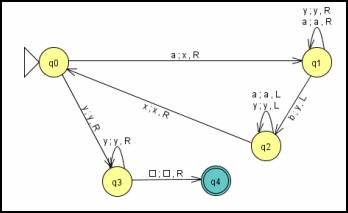
\includegraphics[width=0.5\textwidth]{funcao_de_transicao.jpg}
\caption{\label{fig:funcao_de_transicao}Funções de transição em um conjunto de estados.}
\end{figure}



\subsection{Como funciona uma Maquina de Turing Universal}





























\section{Fodase}
\subsection{Adding photo}

First you have to upload the image file from your computer using the upload link in the file-tree menu. Then use the includegraphics command to include it in your document. Use the figure environment and the caption command to add a number and a caption to your figure. See the code for Figure %\ref{fig:frog}% in this section for an example.

Note that your figure will automatically be placed in the most appropriate place for it, given the surrounding text and taking into account other figures or tables that may be close by. You can find out more about adding images to your documents in this help article on \href{https://www.overleaf.com/learn/how-to/Including_images_on_Overleaf}{including images on Overleaf}.

%\begin{figure}
%\centering
%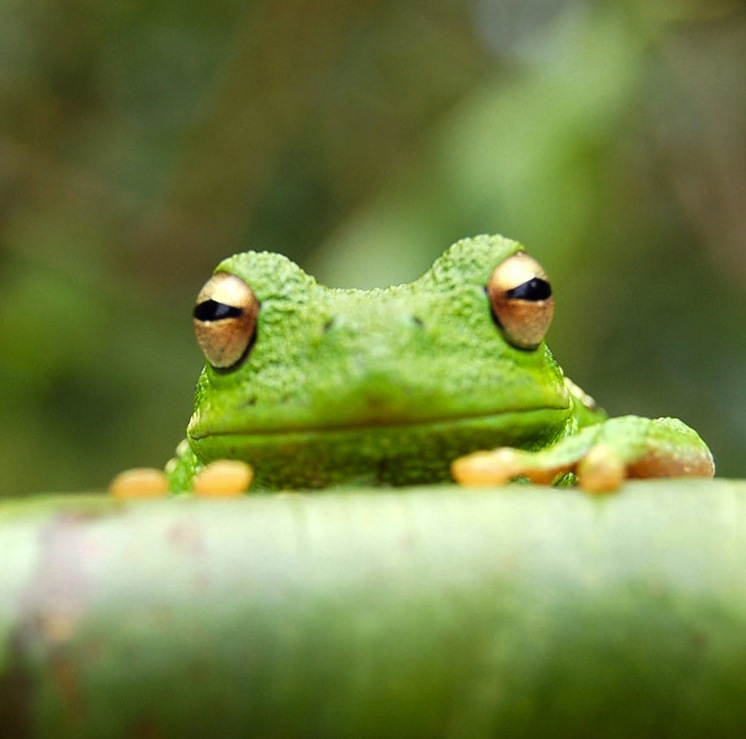
\includegraphics[width=0.3\textwidth]{frog.jpg}
%\caption{\label{fig:frog}This frog was uploaded via the file-tree menu.}
%\end{figure}




\subsection{How to add Tables}

%Use the table and tabular environments for basic tables --- see Table~\ref{tab:widgets}, for example. For more information, please see this help article on \href{https://www.overleaf.com/learn/latex/tables}{tables}. 

%\begin{table}
%\centering
%\begin{tabular}{l|r}
%Item & Quantity \\\hline
%Widgets & 42 \\
%Gadgets & 13
%\end{tabular}
%\caption{\label{tab:widgets}An example table.}
%\end{table}

\subsection{How to add Comments and Track Changes}

Comments can be added to your project by highlighting some text and clicking ``Add comment'' in the top right of the editor pane. To view existing comments, click on the Review menu in the toolbar above. To reply to a comment, click on the Reply button in the lower right corner of the comment. You can close the Review pane by clicking its name on the toolbar when you're done reviewing for the time being.

Track changes are available on all our \href{https://www.overleaf.com/user/subscription/plans}{premium plans}, and can be toggled on or off using the option at the top of the Review pane. Track changes allow you to keep track of every change made to the document, along with the person making the change. 

\subsection{How to add Lists}

You can make lists with automatic numbering \dots

\begin{enumerate}
\item Like this,
\item and like this.
\end{enumerate}
\dots or bullet points \dots
\begin{itemize}
\item Like this,
\item and like this.
\end{itemize}

\subsection{How to write Mathematics}

\LaTeX{} is great at typesetting mathematics. Let $X_1, X_2, \ldots, X_n$ be a sequence of independent and identically distributed random variables with $\text{E}[X_i] = \mu$ and $\text{Var}[X_i] = \sigma^2 < \infty$, and let
\[S_n = \frac{X_1 + X_2 + \cdots + X_n}{n}
      = \frac{1}{n}\sum_{i}^{n} X_i\]
denote their mean. Then as $n$ approaches infinity, the random variables $\sqrt{n}(S_n - \mu)$ converge in distribution to a normal $\mathcal{N}(0, \sigma^2)$.


\subsection{How to change the margins and paper size}

Usually the template you're using will have the page margins and paper size set correctly for that use-case. For example, if you're using a journal article template provided by the journal publisher, that template will be formatted according to their requirements. In these cases, it's best not to alter the margins directly.

If however you're using a more general template, such as this one, and would like to alter the margins, a common way to do so is via the geometry package. You can find the geometry package loaded in the preamble at the top of this example file, and if you'd like to learn more about how to adjust the settings, please visit this help article on \href{https://www.overleaf.com/learn/latex/page_size_and_margins}{page size and margins}.

\subsection{How to change the document language and spell check settings}

Overleaf supports many different languages, including multiple different languages within one document. 

To configure the document language, simply edit the option provided to the babel package in the preamble at the top of this example project. To learn more about the different options, please visit this help article on \href{https://www.overleaf.com/learn/latex/International_language_support}{international language support}.

To change the spell check language, simply open the Overleaf menu at the top left of the editor window, scroll down to the spell check setting, and adjust accordingly.

\subsection{How to add Citations and a References List}

You can simply upload a \verb|.bib| file containing your BibTeX entries, created with a tool such as JabRef. You can then cite entries from it, like this: \cite{greenwade93}. Just remember to specify a bibliography style, as well as the filename of the \verb|.bib|. You can find a \href{https://www.overleaf.com/help/97-how-to-include-a-bibliography-using-bibtex}{video tutorial here} to learn more about BibTeX.

If you have an \href{https://www.overleaf.com/user/subscription/plans}{upgraded account}, you can also import your Mendeley or Zotero library directly as a \verb|.bib| file, via the upload menu in the file-tree.

\subsection{Good luck!}

We hope you find Overleaf useful, and do take a look at our \href{https://www.overleaf.com/learn}{help library} for more tutorials and user guides! Please also let us know if you have any feedback using the Contact Us link at the bottom of the Overleaf menu --- or use the contact form at \url{https://www.overleaf.com/contact}.

\bibliographystyle{alpha}
\bibliography{sample}

\end{document}